%=================================================================
\section{Introduction}\label{sec-intro}



%\todo{The importance of the area}
%\blindtext

Credit card fraud refers to intentional acts of using forged or invalidated credit cards, impersonating others to deceive for financial gain, or engaging in malicious overdraft behavior using one's own credit card. There are three main forms of credit card fraud: card lost or stolen fraud, application fraud, and counterfeit credit card fraud. Among these fraud cases, over 60\% involve counterfeit credit cards, characterized by organized criminal activities that include stealing card information, manufacturing fake cards, selling counterfeit cards, and then using these fake cards to commit crimes for huge profits. Credit card fraud detection is a crucial method for banks to minimize losses.


%\todo{The problems faced by most current methods}
%\blindtext

This article utilizes a dataset sourced from Kaggle to implement credit card fraud detection. The dataset contains transaction information of European cardholders during September 2013, conducted through credit cards. The dataset covers transactions that occurred within a span of two days, with a total of 284,807 transactions. Among these transactions, there were 492 cases of fraud, making the dataset highly imbalanced, where the positive class (fraudulent transactions) accounts for only 0.172% of all transactions.

The original dataset has undergone anonymization and Principal Component Analysis (PCA) processing. The anonymous variables V1, V2, ..., V28 represent the principal components obtained through PCA, and the only variables not subjected to PCA are Time and Amount. Time represents the time elapsed between each transaction and the first transaction in the dataset, measured in seconds, while Amount represents the transaction amount. The "Class" variable is a categorical variable, taking the value 1 when fraud occurs and 0 otherwise.

%\todo{What can be addressed by existing methods; Why those problems are challenges to existing methods?}
%\blindtext

This article utilizes a dataset sourced from Kaggle to implement credit card fraud detection. The dataset contains transaction information of European cardholders during September 2013, conducted through credit cards. The dataset covers transactions that occurred within a span of two days, with a total of 284,807 transactions. Among these transactions, there were 492 cases of fraud, making the dataset highly imbalanced, where the positive class (fraudulent transactions) accounts for only 0.172% of all transactions.


%\todo{What provides the motivation of this work? What are the research issues? What is the rationale of this work? }
%\blindtext

The original dataset has undergone anonymization and Principal Component Analysis (PCA) processing. The anonymous variables V1, V2, ..., V28 represent the principal components obtained through PCA, and the only variables not subjected to PCA are Time and Amount. Time represents the time elapsed between each transaction and the first transaction in the dataset, measured in seconds, while Amount represents the transaction amount. The "Class" variable is a categorical variable, taking the value 1 when fraud occurs and 0 otherwise.

The main implementation in this article is utilizing the Isolation Forest algorithm to achieve credit card fraud detection. By continuously fine-tuning the algorithm through parameter adjustments, the article aims to improve the algorithm's performance.



\section{Method} \label{sec-method}
The Isolation Forest algorithm, proposed in 2008 by Liu Fei, Zhou Zhihua, and others, does not rely on distance or density metrics to describe the differences between samples and other samples. Instead, it directly characterizes the so-called isolation level. Therefore, this algorithm is simple, efficient, and widely used in the industry.

The logic of the Isolation Forest algorithm is intuitive. It uses binary trees to split the data, and both sample selection and feature selection are performed using randomization. If a certain sample is an outlier, it may require very few iterations to be isolated.

Isolation Forest algorithm code is ~\cref{alg:iForest}:
\begin{algorithm}[!h]
	\caption{ \textit{iForest}}
	\label{alg:iForest}
	\renewcommand{\algorithmicrequire}{\textbf{Input:}}
	\renewcommand{\algorithmicensure}{\textbf{Output:}}
	
	\begin{algorithmic}[1]
		\REQUIRE $X$-Input data, $t$-number of trees ,$\varphi$ - subsampling size %%input
		\ENSURE a set of \textit{t iTRees}   %%output
		\STATE $\textbf{Initialize}$ $\textit{Forest}$
		\STATE set height limit $l = ceiling(log_{2}\varphi)$
		
		\FOR{ $i = 1$ to $\textit{t}$} 
		\STATE $X^{\prime}\!\leftarrow\!\cup(\textit{X,$\varphi$})$
		\STATE $\textit{Forest}\!\leftarrow\!\cup\textit{iTRees}(X^{\prime},0,\mathit{l})$
		\ENDFOR
		\RETURN $\textit{Forest}$
	\end{algorithmic}
\end{algorithm}

\section{Data Exploration} \label{sec-exploration}


In this session, basic tools from pandas were utilized to perform data analysis and exploration. By analyzing the data, a more intuitive understanding was gained.

\cref{tbl:data-description}provides a basic overview of the data for each attribute, including measures such as the mean, maximum, minimum, and other indicators.

\begin{table}  \centering
	
	\caption{Data description}
	\label{tbl:data-description}
	\resizebox{\textwidth}{!}
	{
		\begin{tabular}{cccccccccccccccccccccccccccccccc}
			& Time        & V1          & V2          & V3          & V4          & V5          & V6          & V7          & V8          & V9          & V10         & V11         & V12         & V13         & V14         & V15         & V16         & V17         & V18         & V19         & V20         & V21         & V22         & V23         & V24         & V25         & V26         & V27         & V28         & Amount      & Class       \\
			count & 284807.0000 & 284807.0000 & 284807.0000 & 284807.0000 & 284807.0000 & 284807.0000 & 284807.0000 & 284807.0000 & 284807.0000 & 284807.0000 & 284807.0000 & 284807.0000 & 284807.0000 & 284807.0000 & 284807.0000 & 284807.0000 & 284807.0000 & 284807.0000 & 284807.0000 & 284807.0000 & 284807.0000 & 284807.0000 & 284807.0000 & 284807.0000 & 284807.0000 & 284807.0000 & 284807.0000 & 284807.0000 & 284807.0000 & 284807.0000 & 284807.0000 \\
			mean  & 94813.8596  & 0.0000      & 0.0000      & 0.0000      & 0.0000      & 0.0000      & 0.0000      & 0.0000      & 0.0000      & 0.0000      & 0.0000      & 0.0000      & 0.0000      & 0.0000      & 0.0000      & 0.0000      & 0.0000      & 0.0000      & 0.0000      & 0.0000      & 0.0000      & 0.0000      & 0.0000      & 0.0000      & 0.0000      & 0.0000      & 0.0000      & 0.0000      & 0.0000      & 88.3496     & 0.0017      \\
			std   & 47488.1460  & 1.9587      & 1.6513      & 1.5163      & 1.4159      & 1.3802      & 1.3323      & 1.2371      & 1.1944      & 1.0986      & 1.0888      & 1.0207      & 0.9992      & 0.9953      & 0.9586      & 0.9153      & 0.8763      & 0.8493      & 0.8382      & 0.8140      & 0.7709      & 0.7345      & 0.7257      & 0.6245      & 0.6056      & 0.5213      & 0.4822      & 0.4036      & 0.3301      & 250.1201    & 0.0415      \\
			min   & 0.0000      & -56.4075    & -72.7157    & -48.3256    & -5.6832     & -113.7433   & -26.1605    & -43.5572    & -73.2167    & -13.4341    & -24.5883    & -4.7975     & -18.6837    & -5.7919     & -19.2143    & -4.4989     & -14.1299    & -25.1628    & -9.4987     & -7.2135     & -54.4977    & -34.8304    & -10.9331    & -44.8077    & -2.8366     & -10.2954    & -2.6046     & -22.5657    & -15.4301    & 0.0000      & 0.0000      \\
			0.25  & 54201.5000  & -0.9204     & -0.5985     & -0.8904     & -0.8486     & -0.6916     & -0.7683     & -0.5541     & -0.2086     & -0.6431     & -0.5354     & -0.7625     & -0.4056     & -0.6485     & -0.4256     & -0.5829     & -0.4680     & -0.4837     & -0.4988     & -0.4563     & -0.2117     & -0.2284     & -0.5424     & -0.1618     & -0.3546     & -0.3171     & -0.3270     & -0.0708     & -0.0530     & 5.6000      & 0.0000      \\
			0.5   & 84692.0000  & 0.0181      & 0.0655      & 0.1798      & -0.0198     & -0.0543     & -0.2742     & 0.0401      & 0.0224      & -0.0514     & -0.0929     & -0.0328     & 0.1400      & -0.0136     & 0.0506      & 0.0481      & 0.0664      & -0.0657     & -0.0036     & 0.0037      & -0.0625     & -0.0295     & 0.0068      & -0.0112     & 0.0410      & 0.0166      & -0.0521     & 0.0013      & 0.0112      & 22.0000     & 0.0000      \\
			0.75  & 139320.5000 & 1.3156      & 0.8037      & 1.0272      & 0.7433      & 0.6119      & 0.3986      & 0.5704      & 0.3273      & 0.5971      & 0.4539      & 0.7396      & 0.6182      & 0.6625      & 0.4931      & 0.6488      & 0.5233      & 0.3997      & 0.5008      & 0.4589      & 0.1330      & 0.1864      & 0.5286      & 0.1476      & 0.4395      & 0.3507      & 0.2410      & 0.0910      & 0.0783      & 77.1650     & 0.0000      \\
			max   & 172792.0000 & 2.4549      & 22.0577     & 9.3826      & 16.8753     & 34.8017     & 73.3016     & 120.5895    & 20.0072     & 15.5950     & 23.7451     & 12.0189     & 7.8484      & 7.1269      & 10.5268     & 8.8777      & 17.3151     & 9.2535      & 5.0411      & 5.5920      & 39.4209     & 27.2028     & 10.5031     & 22.5284     & 4.5845      & 7.5196      & 3.5173      & 31.6122     & 33.8478     & 25691.1600  & 1.0000     
		\end{tabular}
	}
\end{table}

From the perspective of fraud occurrence, the data was visualized as shown in \cref{fig:fraud data}. It can be observed that the instances of fraud are significantly fewer than non-fraudulent cases, indicating the presence of data imbalance.

\begin{figure}[H]
	\centering
	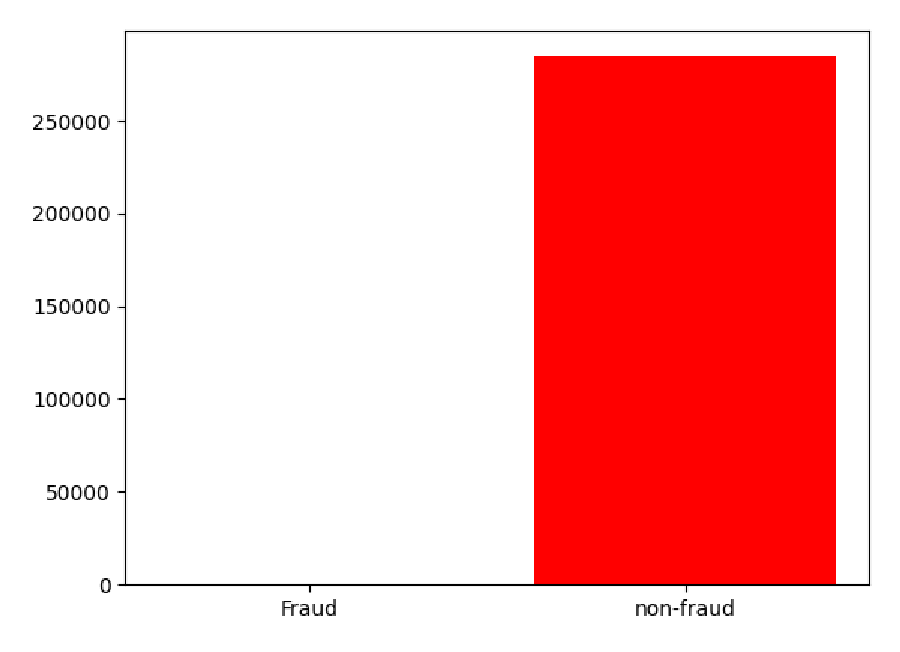
\includegraphics[width=0.7\textwidth]{figures/fraud.eps}
	\caption{fraud or no fraud}
	\label{fig:fraud data}
\end{figure}

\cref{fig:correlation} is a heatmap of correlations, representing the correlation of each attribute with fraud.From the figure, it can be seen that the individual attributes have a relatively low impact on the class, and some even exhibit negative correlations.

\begin{figure}[H]
	\centering
	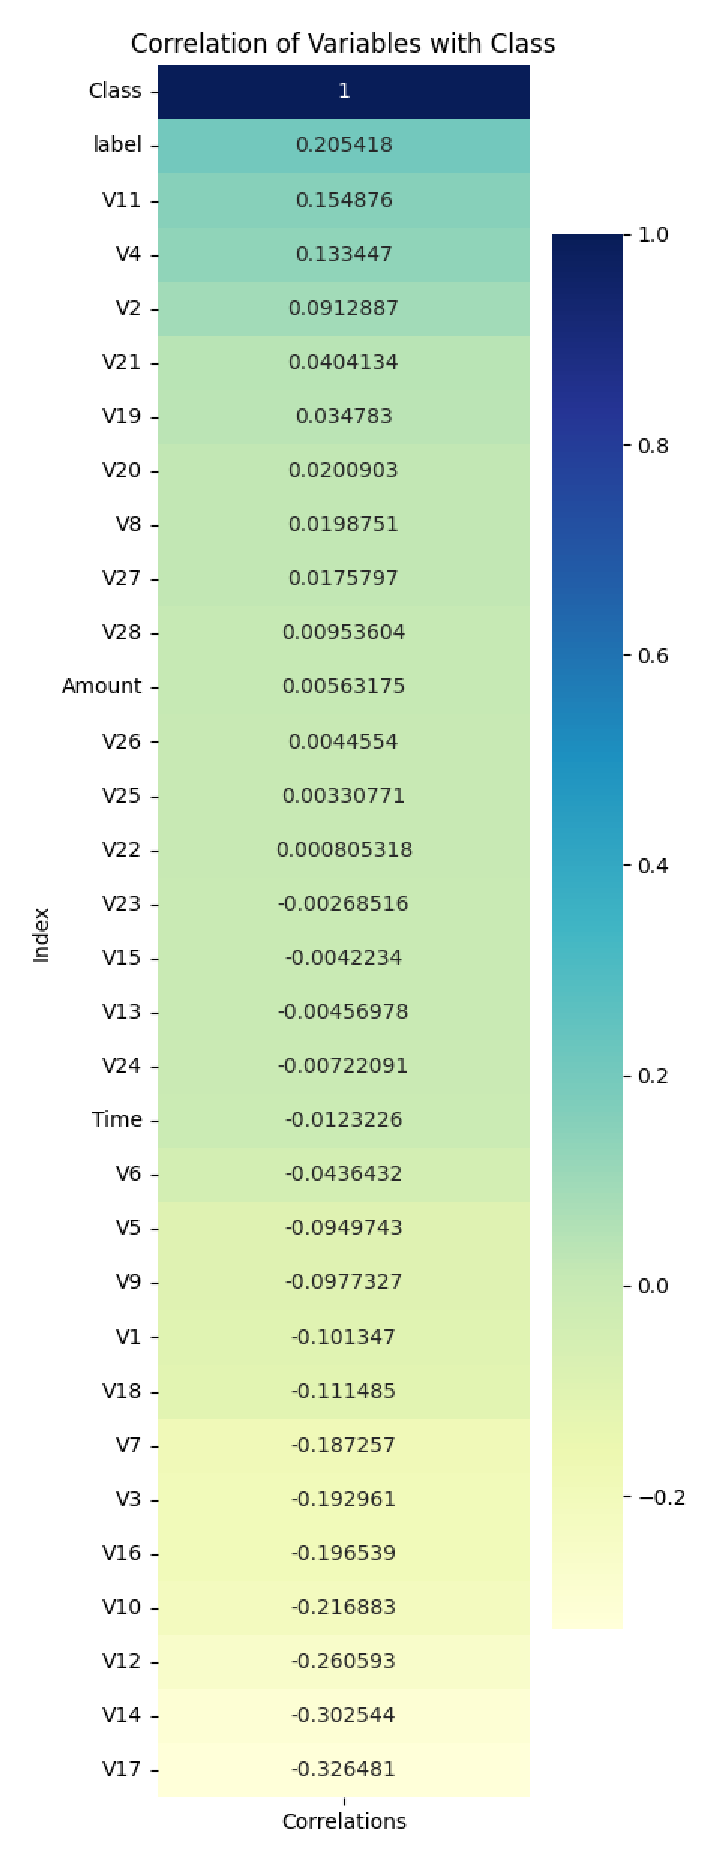
\includegraphics[height=0.5\textheight]{figures/correlation.eps}
	\caption{correlation heat plot}
	\label{fig:correlation}
\end{figure}




\section{Experiment} \label{sec-experiment}
In the experimental design, we achieved the optimal performance of the model by continuously adjusting parameters. The evaluation of the training set's accuracy and recall mainly involved removing attributes and continuously changing the parameters of the isolation forest.

\begin{table}\centering
	
	\caption{parameter adjustment}
	\label{tbl:parameter-adjustment}
	\resizebox{\textwidth}{!}{
		\begin{tabular}{cccccc}
			\toprule
			Parameter & Accuarcy & Recall & Parameter & Accuarcy & Recall\\
			\midrule
			none-parameter-adjust & 0.963 & 0.821  & none-parameter-adjust(feature \_delete) & 0.953 & 0.663 \\
			n\_estimators-adjust(220) & 0.981 & 0.722  & n\_estimators-adjust(feature \_delete)(140) & 0.980 & 0.520 \\
			n\_features-adjust(11) & 0.981 & 0.750  & n\_features-adjust(feature \_delete)(11) & 0.981 & 0.522 \\
			max\_samples-adjust & 0.981 & 0.829  & nmax\_samples-adjust(feature \_delete) & 0.980 & 0.634\\
			\bottomrule
		\end{tabular}
	}
\end{table}

\cref{tbl:parameter-adjustment} displays the accuracy and recall rates under various parameter adjustments. From the table, it can be observed that the recall rate deteriorates after removing some features. This implies that although these features may exhibit negative correlations with the outcome, they should not be indiscriminately deleted. By iteratively trying different parameter combinations, we ultimately identified the optimal parameters.

\cref{fig:fig_n_estimators} and \cref{fig:n_features-adjust}  and \cref{fig:max_samples-adjust} are visualizations of specific parameter adjustments. 
\begin{figure}
	\centering
	\subfigure[n\_estimators-adjust]{
		\begin{minipage}[b]{0.4\textwidth}
			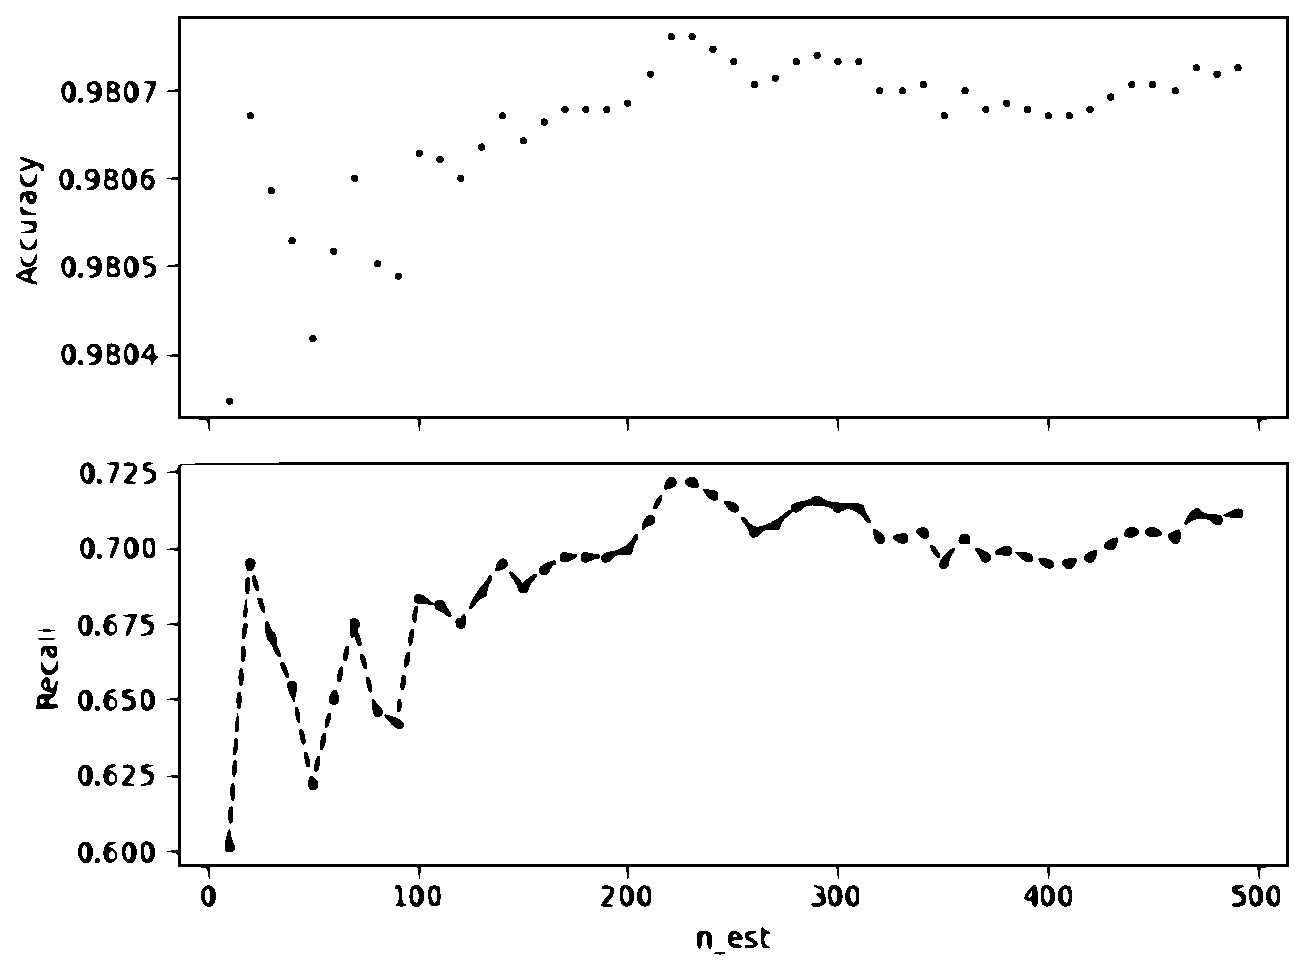
\includegraphics[width=1\textwidth]{figures/n_est_node.eps}
		\end{minipage}
		\label{fig:hor_2figs_1cap_2subcap_1}
	}
	\subfigure[n\_estimators-adjust (feature\_delete)]{
		\begin{minipage}[b]{0.4\textwidth}
			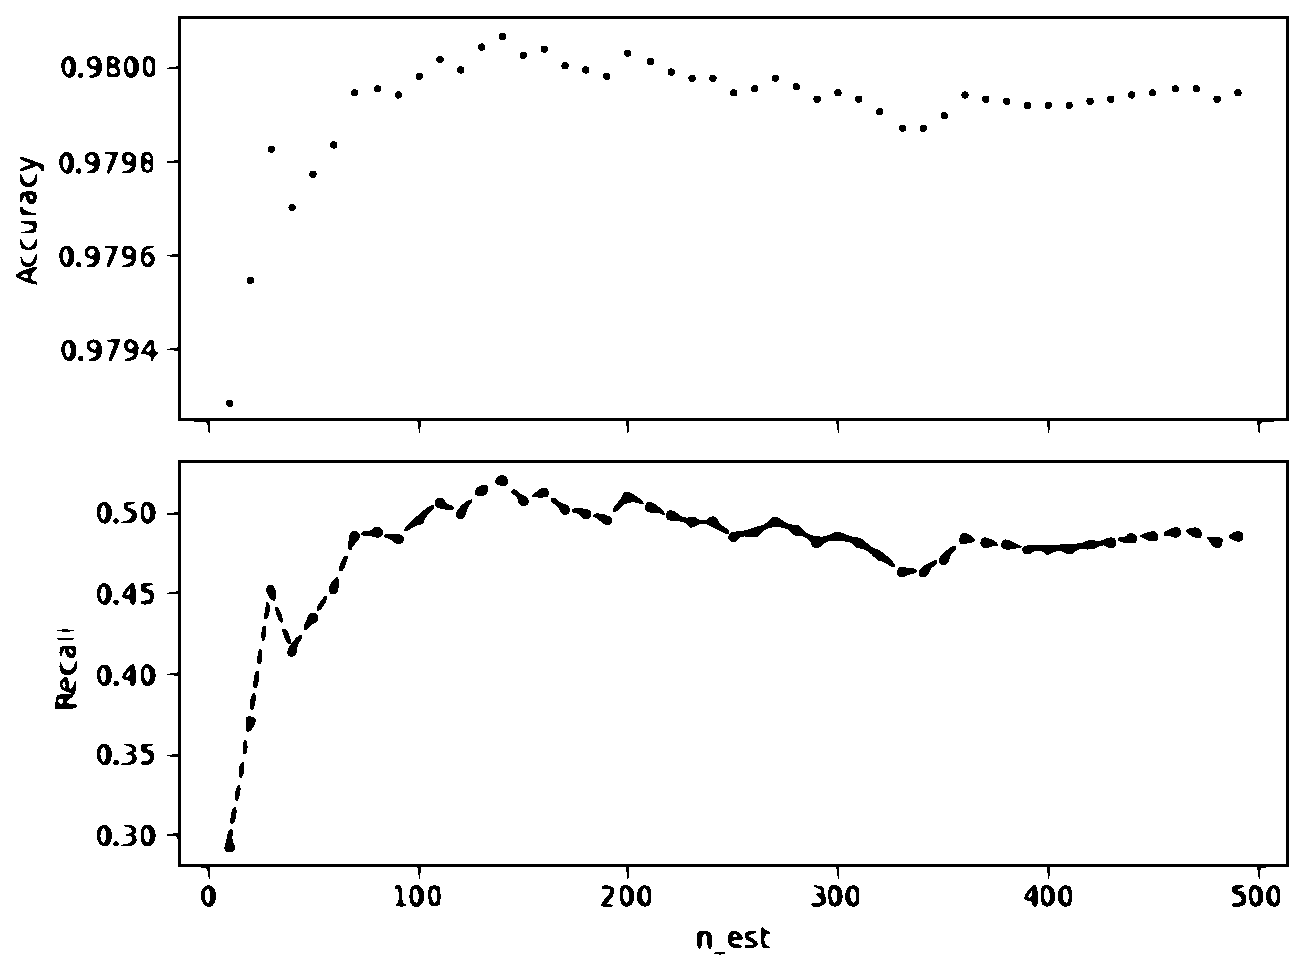
\includegraphics[width=1\textwidth]{figures/n_est.eps}
		\end{minipage}
		\label{fig:hor_2figs_1cap_2subcap_2}
	}
	\caption{n\_estimators-adjust}
	\label{fig:fig_n_estimators}
\end{figure}

\begin{figure}
	\centering
	\subfigure[n\_features-adjust]{
		\begin{minipage}[b]{0.4\textwidth}
			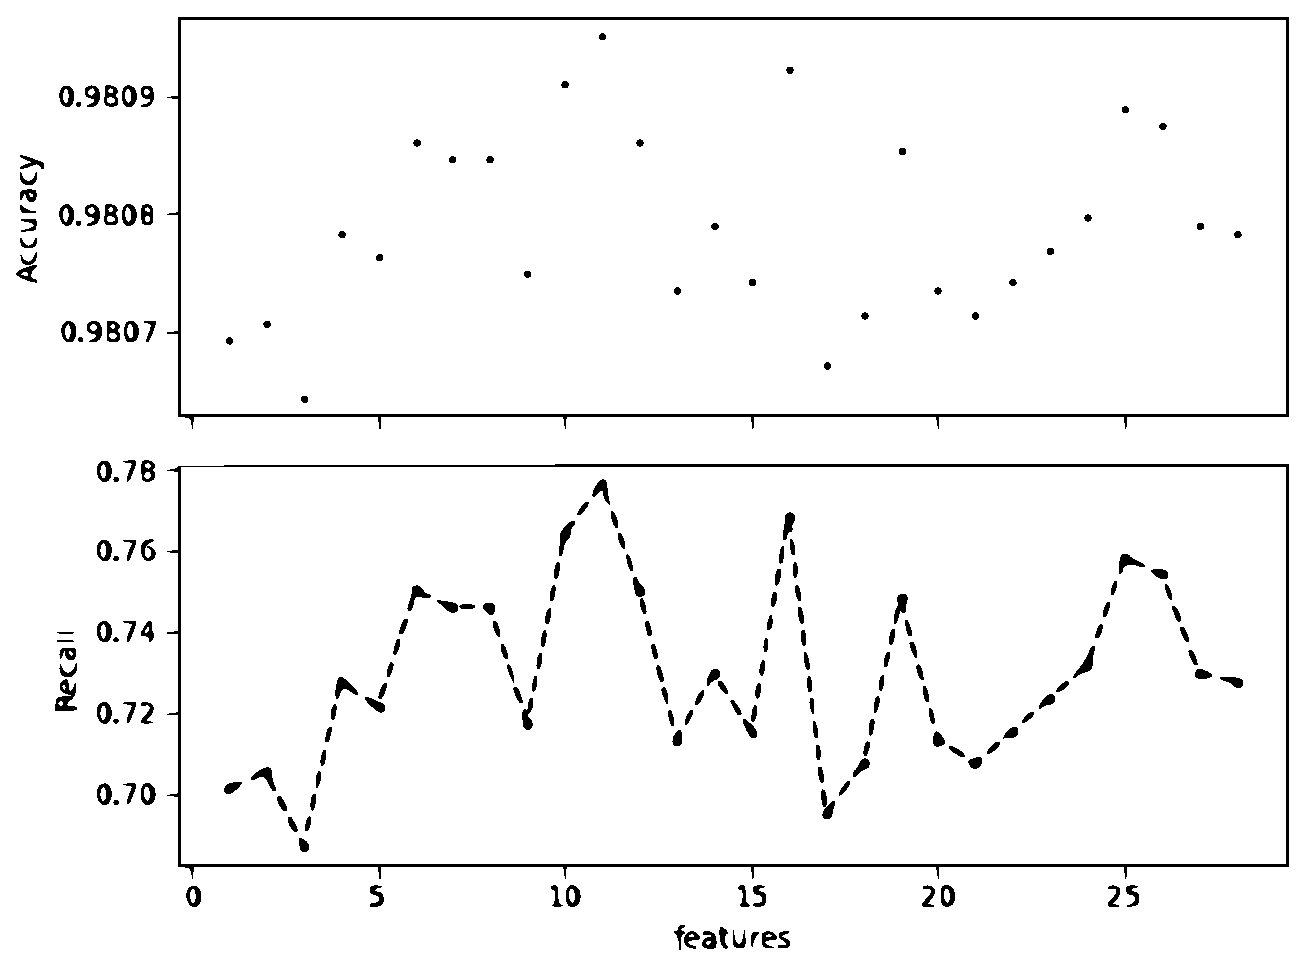
\includegraphics[width=1\textwidth]{figures/feature_nodelete.eps}
		\end{minipage}
		\label{fig:hor_2}
	}
	\subfigure[n\_features-adjust (feature\_delete)]{
		\begin{minipage}[b]{0.4\textwidth}
			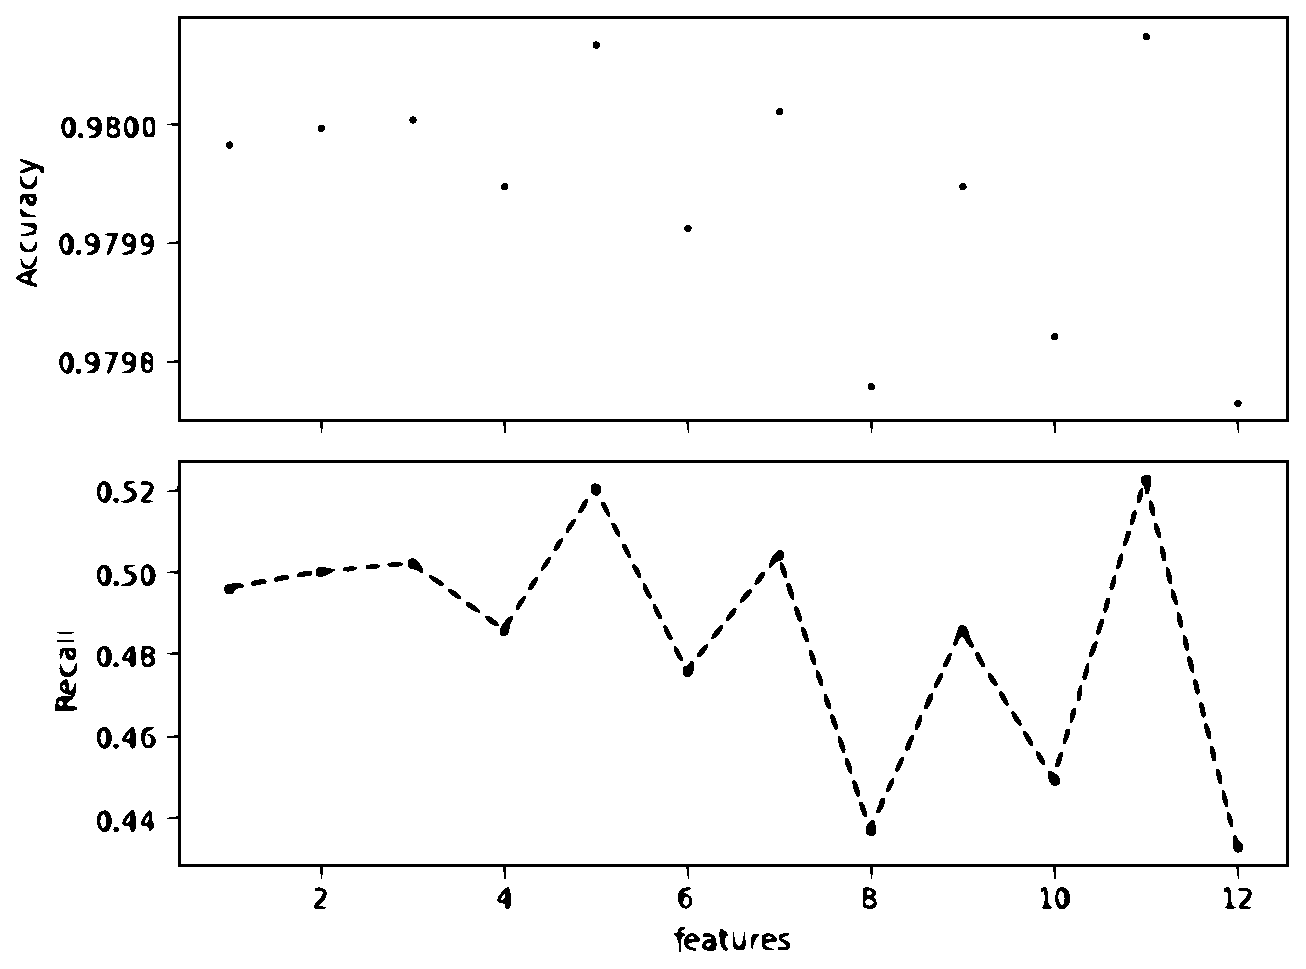
\includegraphics[width=1\textwidth]{figures/feature.eps}
		\end{minipage}
		\label{fig:hor}
	}
	\caption{n\_efeatures-adjust}
	\label{fig:n_features-adjust}
\end{figure}

\begin{figure}
	\centering
	\subfigure[max\_samples-adjust]{
		\begin{minipage}[b]{0.4\textwidth}
			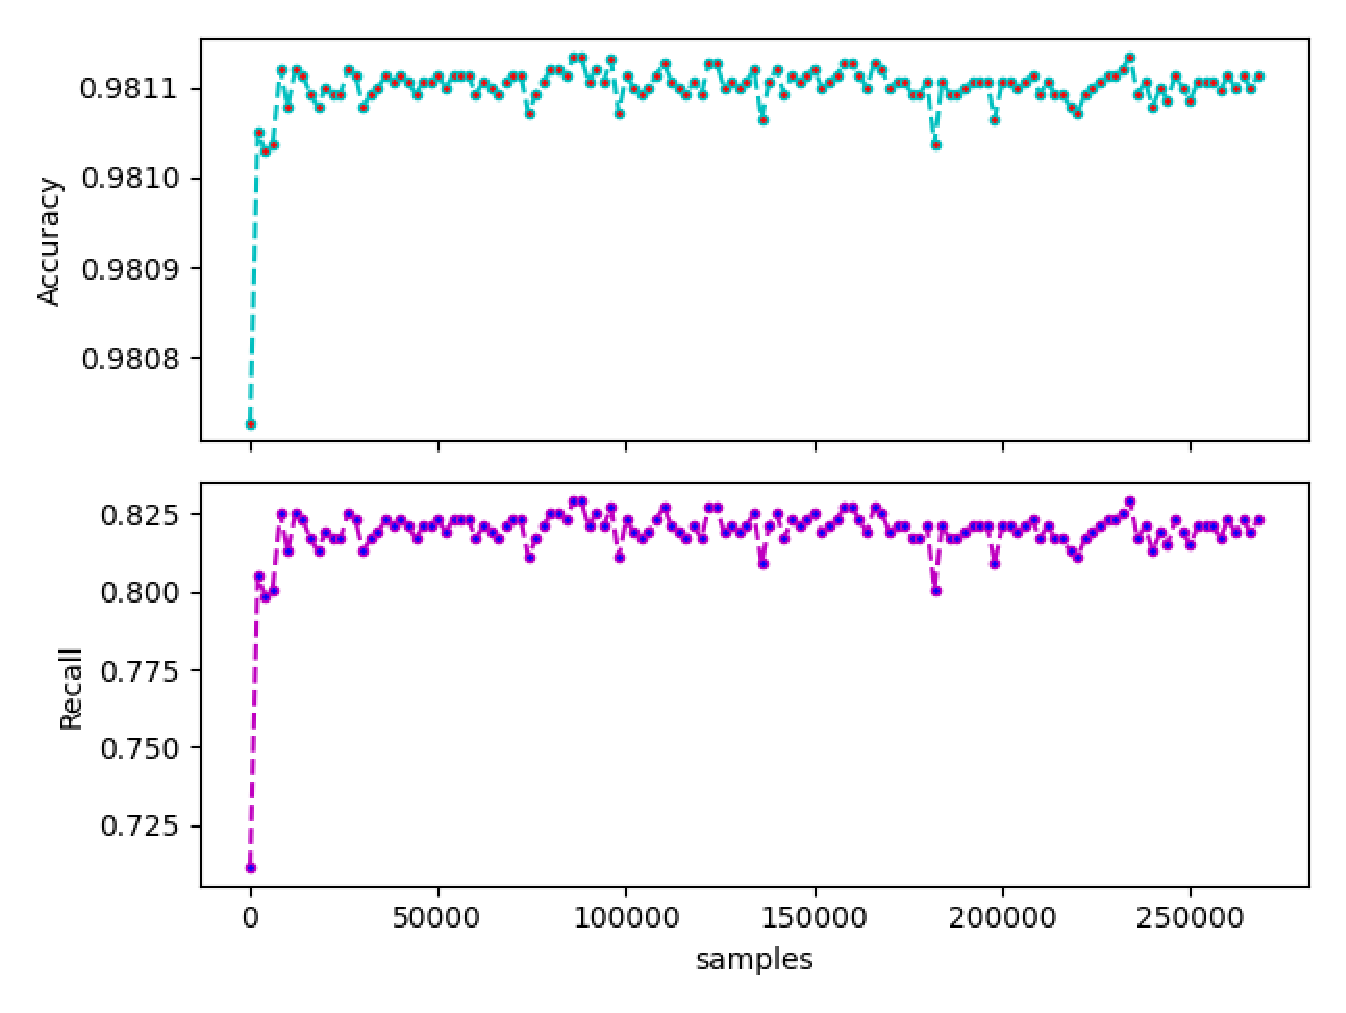
\includegraphics[width=1\textwidth]{figures/max_exampleN.eps}
		\end{minipage}
		\label{fig:h}
	}
	\subfigure[max\_samples-adjust (feature\_delete)]{
		\begin{minipage}[b]{0.4\textwidth}
			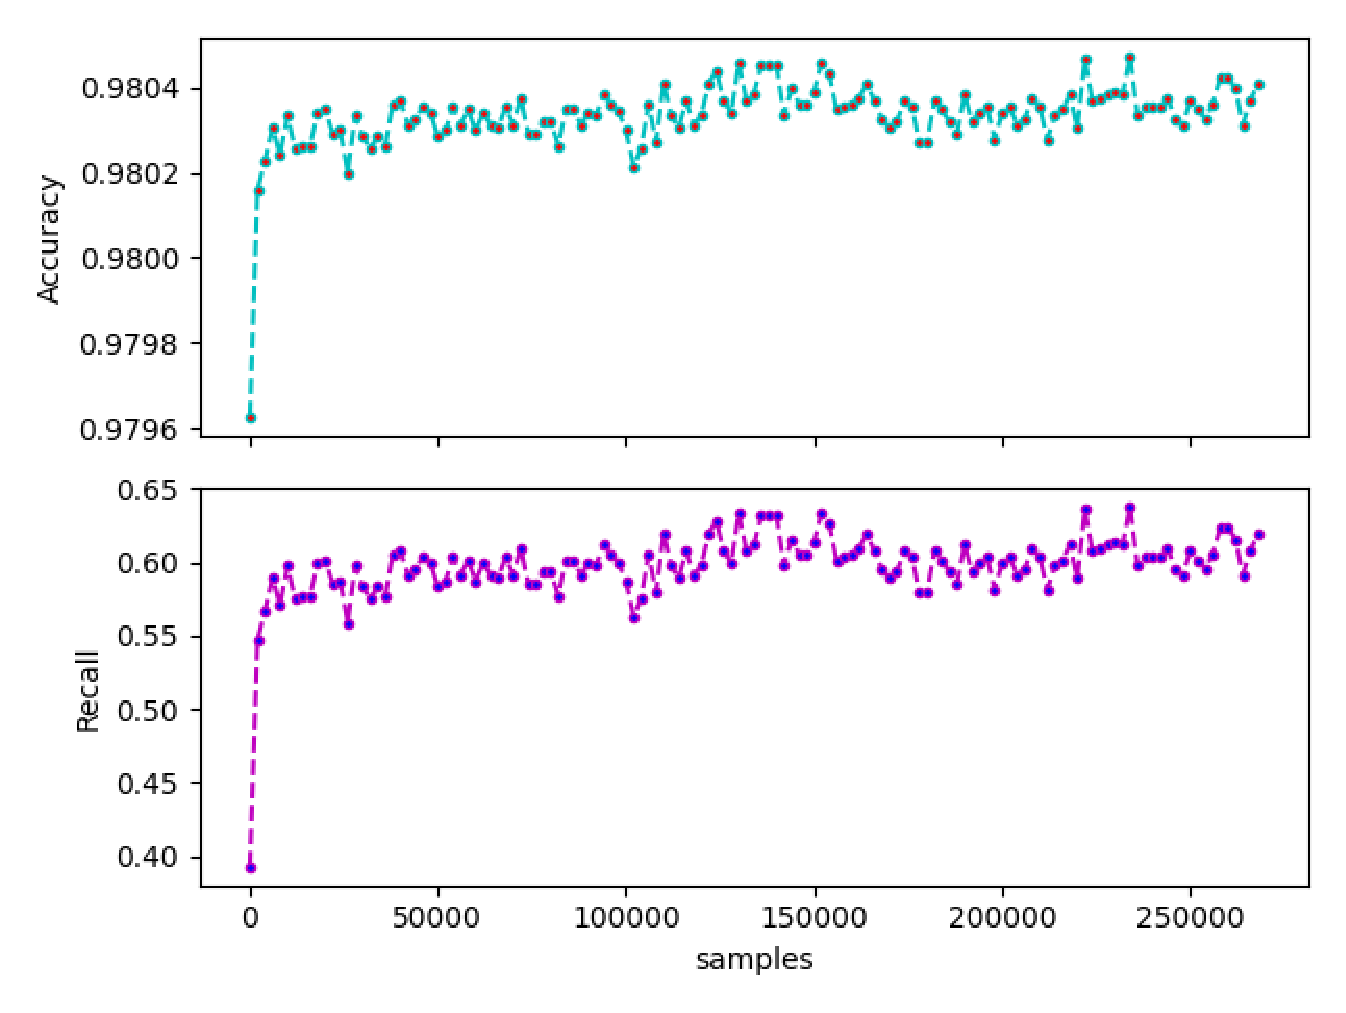
\includegraphics[width=1\textwidth]{figures/max_example.eps}
		\end{minipage}
		\label{fig:ho}
	}
	\caption{max\_samples-adjust}
	\label{fig:max_samples-adjust}
\end{figure}

\section{Conclusions} \label{sec-conclusions}

The detection of credit card fraud data was achieved through Isolation Forest, and by continuously adjusting the parameters of the algorithm, a high level of accuracy and recall was ultimately reached, at 0.98 and 0.8, respectively.

However, a notable drawback of this method is the lack of a more in-depth analysis of attributes. This could mean that in the data preprocessing stage or feature selection process, there was insufficient exploration, understanding, and utilization of attribute information relevant to fraud. While optimizing the accuracy and recall of the model is undoubtedly important, equal attention should also be given to the importance and correlation of attributes, as well as their role in fraud detection.


